\section{Results}
\label{sec:results}

In this section, we provide relevant details pertaining to the construction of the surrogate for the field of interest, i.e. the
residual stress in the AM part cross-section using the PCAS method in~\ref{sub:surr}. The surrogate is used to map
the process control parameters and the material properties to the residual stress field. The computational efficiency
enabled by the surrogate is exploited to perform a global sensitivity analysis of the inputs in~\ref{sub:gsa}. Finally, the
surrogate is used for reliability prediction for the AM part by estimating the probability of failure based on residual stress
in~\ref{sub:reliability}.

\subsection{Surrogate Model}
\label{sub:surr}

A surrogate model is constructed for the residual stress field at the cross-section of the part 
(x-z plane in Figure~\ref{fig:PartwMesh}) passing through its center. The surrogate maps three sets of
parameters, namely, the process control parameters~($\bm{\theta_p}$), mechanical properties~($\bm{\theta_m}$),
and thermal properties~($\bm{\theta_t}$) to the stress field. The set of process control parameters includes
the beam power~($P$), scan speed~($v$), and the pre-heat temperature~($T_0$). Mechanical properties
include the yield strength~($Y$), the elastic modulus~($E$), and the bulk density~($\rho$). Thermal 
properties include specific heat~($C_p$) and bulk thermal conductivity~($\kappa$). Note that $C_p$ and $\kappa$
are considered to be functions of the local temperature, $T$. Specifically, a polynomial of degree 2 was fit
to a set of data pertaining to the variation of $C_p$ and $\kappa$ with temperature (20~K--1655~K), 
provided in~\cite{Fu:2014} as shown in Figure~\ref{fig:Cp_kappa}.
%
\begin{figure}[htbp]
\begin{center}
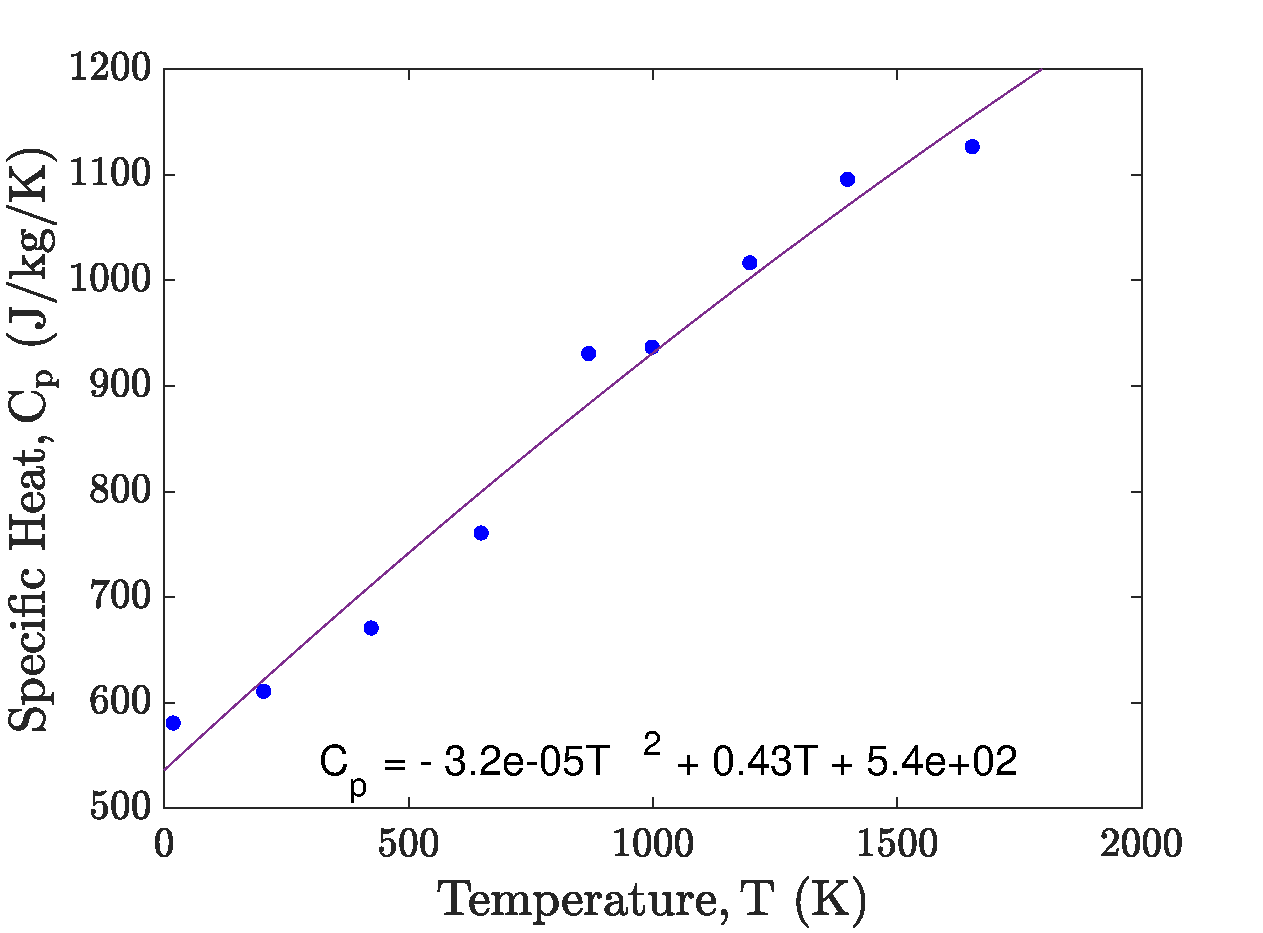
\includegraphics[width=0.42\textwidth]{./Figures/cp_fit}
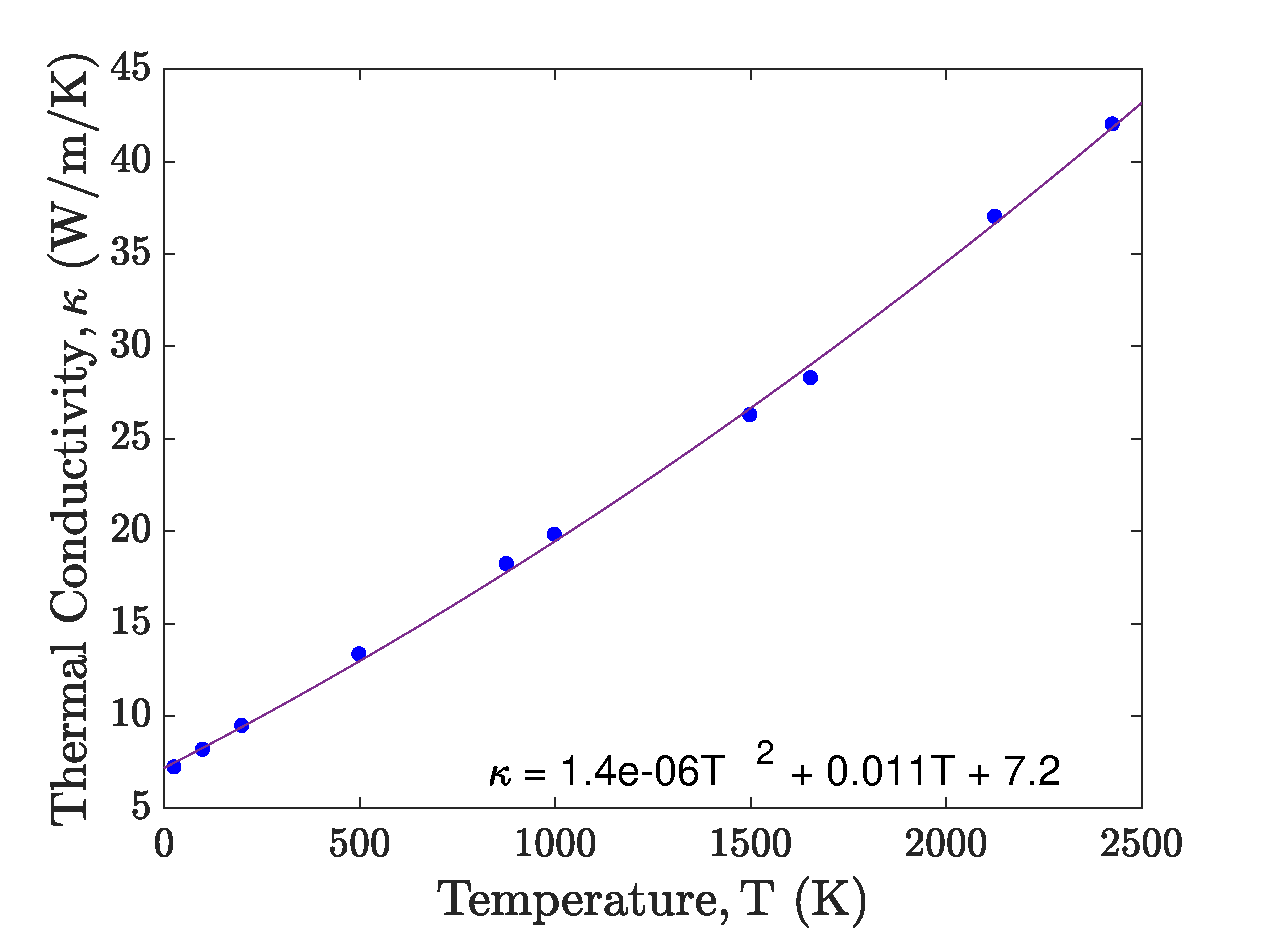
\includegraphics[width=0.42\textwidth]{./Figures/kappa_fit}
\end{center}
\caption{A second degree polynomial fit to specific heat~($C_p$), and thermal conductivity~($\kappa$) data
for a temperature range, [20,1655](K). Note that the data provided in~\cite{Fu:2014} was used to determine
the coefficients of the regression fit.}
\label{fig:Cp_kappa}
\end{figure}
%
Hence, a total of 12 parameters~($\bm{\theta}$) are mapped to the stress field including coefficients of the polynomial fits
corresponding to $C_p$ and $\kappa$. A uniform prior: $\[0.9\bm{\theta^\ast}, 1.1\bm{\theta^\ast}\]$, where $\bm{\theta^\ast}$
denotes a vector of nominal values,
was considered for each parameter. Nominal values of the mechanical properties: $Y$, $E$, and $\rho$ are provided
in Table~\ref{tab:matProp}. Nominal values of the process control parameters and temperature coefficients for
the thermal properties are provided in Table~\ref{tab:remain}.
%
\begin{table}[htbp]
\centering
\caption{EBM process control parameters and temperature coefficients for $C_p$~($C_i$'s) and $\kappa$~($D_i$'s).}
\label{tab:remain}
\vspace{1mm}
\begin{tabular}{ ll }
\toprule
Scan Speed, $v$~(mm/s) & 500 \\
Beam Power, $P$~(W) & 160 \\
Pre-heat Temperature, $T_0$~(C) & 650 \\
Specific heat, $C_p$ = $C_0+C_1T+C_2T^2$~(J/kg/K) & 540~($C_0$),0.43~($C_1$),$-3.2\times 10^{-5}$~($C_2$) \\
Thermal Conductivity, $\kappa$ = $D_0+D_1T+D_2T^2$~(W/m/K) & 7.2~($D_0$),0.011~($D_1$),$1.4\times 10^{-6}$~($D_2$) \\
\bottomrule
\end{tabular}
\end{table}
%%%

Residual stress data was generated 



%The first step in the PCAS
%method involves dimension reduction in the output space using principal component analysis. 


\subsection{Global Sensitivity Analysis}
\label{sub:gsa}


\subsection{Reliability Prediction}
\label{sub:reliability}




 
